\chapter{Benchmark}
\label{cha:benchmark}

\begin{itemize}
	\item LFR-Benchmark Generator
\end{itemize}

\section{Testumgebung}

\subsection{Datens�tze}

\begin{figure}[h] 
	\centering
		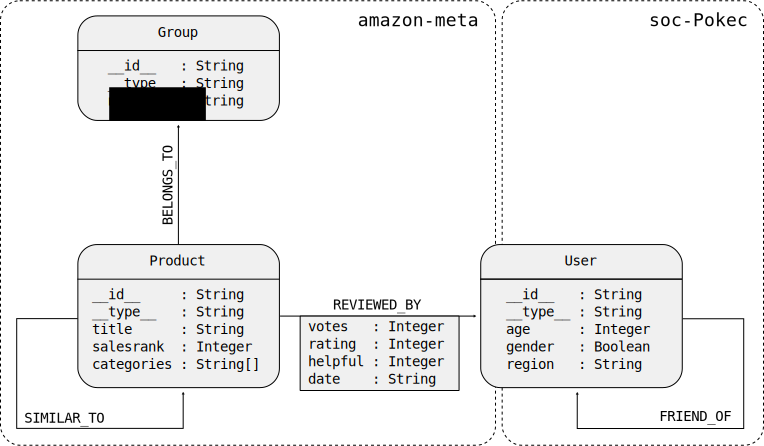
\includegraphics[scale=.75]{schema.pdf}
	\caption[Benchmark: Schema Testdaten]{Schema}
	\label{fig:test}
\end{figure}

\begin{itemize}
	\item Verwendung von ERPNext Schema + Daten (multiplizieren)	
\end{itemize}

\subsection{Testsystem}

\subsection{Methodik}

siehe \cite{Dominguez-Sal2011}

\section{Messungen}

\subsection{Speicherverbrauch}

\subsection{Antwortzeiten}

\begin{itemize}
\item Vergleich Zeichenketten vs. Integer
\end{itemize}

\begin{itemize}
	\item Formulieren verschiedener einfacher und komplexer Anfragen
	\begin{itemize}
		\item Auswahl zuf�lliger Knoten und Abfragen aller Nachbarn bis Tiefe n
		\item Berechnung des Profits in bestimmten Zeitr�umen / Regionen
		\item Auswahl zwei zuf�lliger Knoten vom Typ User, Invoice + Berechnen aller Pfade
		\item ...
	\end{itemize}
\end{itemize}

\section{Ergebnisse}
